\documentclass[10pt]{article}
\usepackage[pdftex]{graphicx, color}
\usepackage{listings}
\usepackage{amsmath}


\usepackage{tikz}
\usetikzlibrary{automata,positioning}

\headheight 8pt \headsep 20pt \footskip 30pt
\textheight 9in \textwidth 6.5in
\oddsidemargin 0in \evensidemargin 0in
\topmargin -.35in

\newcommand {\pts}[1]{({\bf #1 pts})}
\lstset{basicstyle=\small\ttfamily,breaklines=true}

\begin{document}
\begin{center}
\Large CS131 Compilers: Writing Assignment 1\\Due Tuesday, March 27, 2018 at 23:55
\end{center}

\begin{center}
%% Change this:
\LARGE Zhiqiang Xie - 77892769
\end{center}


This assignment asks you to prepare written answers to questions on
regular languages, finite automata, and lexical analysis.  Each of the
questions has a short answer.  You may discuss this assignment with
other students and work on the problems together.  However, your
write-up should be your own individual work and you should indicate in your submission who you worked
with, if applicable. You should use the Latex template provided at the course web site to write your solution and use the \emph{tikz} package to draw
automata.

\begin{center}
%% Change this:
I worked with: (Name,ID), (Name,ID)...
\end{center}

\begin{enumerate}
  \item \pts{$2\times 3=6$} For each of the follow prompts, write any non-empty sentence:
  \begin{enumerate}
           \item Name one reason why you would like to learn in this class.
           \\
            I want to have a comprehensive understanding towards how a program
            worked from coding level to hardware level. So that I can find my
            interest from the whole computer science. \\
            Besides, I'm interested in some topics will be covered
            in this course: intermediate representation, some basic ideas to
            process formal language (since I have some research experience in
            data-driven processing approach, I think there are some good ideas
            can be found from the classical methods)
           \item Write a question you would like the professor to answer �� on any topic, from personal opinions to the class material.
            \\
            What do you think about the key ideas in compilers?\\
            We all know there are some great ideas like cache, intermediate layer in many fields of computer science.
            what's that in computer?
           \item What do you expect from this class.
           \\
           More about IR and some more general approach instead of focusing on
           string and tokens processing too much. Or there's some great general
           ideas hidden in it, that's the question above.
  \end{enumerate}
  %
  \item \pts{$2\times 4=8$} Write regular expressions for the following languages over the alphabet $\Sigma=\{0,1\}$:
 \begin{enumerate}
           \item $L_1$: The set of all finite strings containing only three $1's$.
            \[
            L_1 = (0^*1)\{3\}0^*
            \]
           \item $L_2$: The set of all finite strings containing at least three $1's$ and the third character from beginning is $1$.
            \[
            L_2 = 111[01]^*|(10|01)1(0^*10^*)^+|001(0^*1)\{2,\}0^*
            \]
           \item $L_3$: The set of all finite strings containing at most three $0's$ and at least two $1's$.
           \\
           \begin{align*}
               L_3 =& 0001\{2,\} | 00101^+ | 001\{2,\}(01^*)? | 01001^+
                       | 0101^+(01^*)? | 01\{2,\}(01^*)\{0,2\} | 10001^+ \\
                    &  | 1001^+(01^*)? | 101^+(01^*)\{0,2\} | 1\{2,\}(01^*)\{0,3\}
            \end{align*}
           \item $L_4$: The set of all finite strings which does not contain subsequence $100$.
            \[
            L_4 = 0^*(1^+0)^*1^*
            \]
   \end{enumerate}
   %This example illustrates that regular languages are closed under intersection. Note that
   %$L_3=L_1\cap L_2$.

  \newpage
   \item \pts{$2\times 4=8$} Draw DFA's for each of the languages $L_1$, $L_2$, $L_3$ and $L_4$ from Question 1.
  \begin{enumerate}
    \item $L_1$.
    \\
    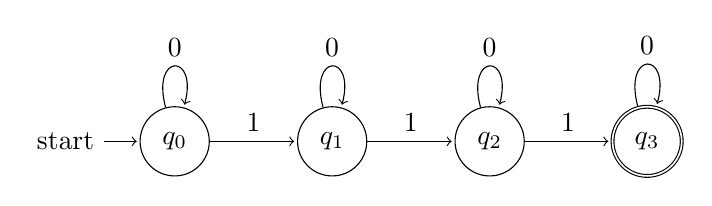
\begin{tikzpicture}[shorten >=1pt,node distance=2cm,on grid,auto]

        \node[state,initial]    (q_0) {$q_0$};
        \node[state]            (q_1) [right of=q_0] {$q_1$};
        \node[state]            (q_2) [right of=q_1] {$q_2$};
        \node[state,accepting]  (q_3) [right of=q_2] {$q_3$};

        \path [->]
              (q_0) edge    [loop above]    node {$0$} (q_0)
              (q_0) edge                    node {$1$} (q_1)
              (q_1) edge    [loop above]    node {$0$} (q_1)
              (q_1) edge                    node {$1$} (q_2)
              (q_2) edge    [loop above]    node {$0$} (q_2)
              (q_2) edge                    node {$1$} (q_3)
              (q_3) edge    [loop above]    node {$0$} (q_3)
              ;

    \end{tikzpicture}
    \item $L_2$.
    \\
    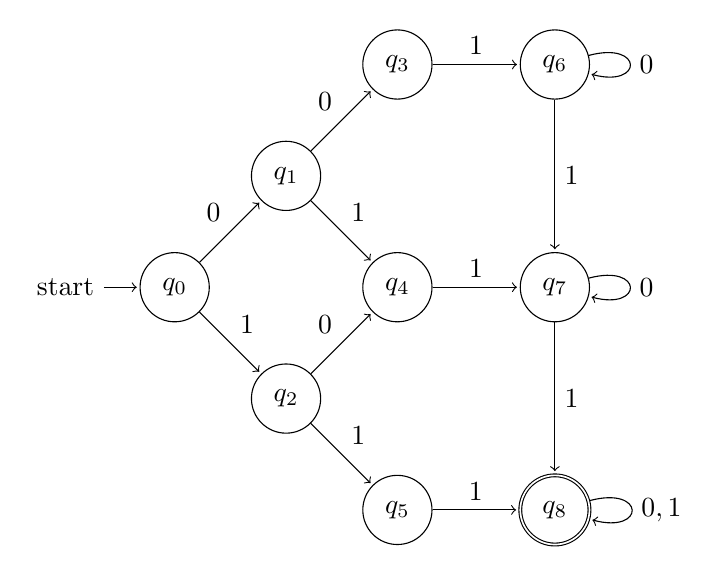
\begin{tikzpicture}[shorten >=1pt,node distance=2cm,on grid,auto]
        \node[state,initial]    (q_0)   {$q_0$};
        \node[state]            (q_1) [above right=of q_0] {$q_1$};
        \node[state]            (q_2) [below right=of q_0] {$q_2$};
        \node[state]            (q_3) [above right=of q_1] {$q_3$};
        \node[state]            (q_4) [below right=of q_1] {$q_4$};
        \node[state]            (q_5) [below right=of q_2] {$q_5$};
        \node[state]            (q_6) [right=of q_3] {$q_6$};
        \node[state]            (q_7) [right=of q_4] {$q_7$};
        \node[state, accepting] (q_8) [right=of q_5] {$q_8$};
        \path[->]
        (q_0)   edge  node  {$0$} (q_1)
                edge  node  {$1$} (q_2)
        (q_1)   edge  node  {$0$} (q_3)
                edge  node  {$1$} (q_4)
        (q_2)   edge  node  {$0$} (q_4)
                edge  node  {$1$} (q_5)
        (q_3)   edge  node  {$1$} (q_6)
        (q_4)   edge  node  {$1$} (q_7)
        (q_5)   edge  node  {$1$} (q_8)
        (q_6)   edge  node  {$1$} (q_7)
                edge  [loop right]  node  {$0$}  ()
        (q_7)   edge  node  {$1$} (q_8)
                edge  [loop right]  node  {$0$}  ()
        (q_8)   edge  [loop right]  node  {$0,1$}  ()
        ;
    \end{tikzpicture}
    \item $L_3$.
    \\
    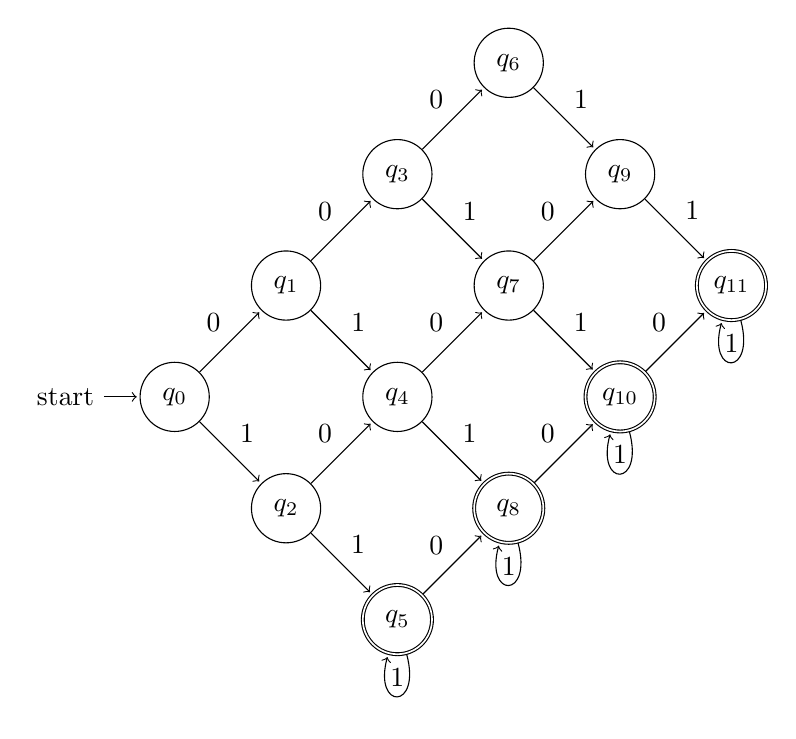
\begin{tikzpicture}[shorten >=1pt,node distance=2cm,on grid,auto]
        \node[state,initial]    (q_0)   {$q_0$};
        \node[state]            (q_1) [above right=of q_0] {$q_1$};
        \node[state]            (q_2) [below right=of q_0] {$q_2$};
        \node[state]            (q_3) [above right=of q_1] {$q_3$};
        \node[state]            (q_4) [below right=of q_1] {$q_4$};
        \node[state,accepting]  (q_5) [below right=of q_2] {$q_5$};
        \node[state]            (q_6) [above right=of q_3] {$q_6$};
        \node[state]            (q_7) [above right=of q_4] {$q_7$};
        \node[state, accepting] (q_8) [above right=of q_5] {$q_8$};
        \node[state]            (q_9) [above right=of q_7] {$q_9$};
        \node[state, accepting] (q_10) [above right=of q_8] {$q_{10}$};
        \node[state, accepting] (q_11) [below right=of q_9] {$q_{11}$};
        \path[->]
        (q_0)   edge  node  {$0$} (q_1)
                edge  node  {$1$} (q_2)
        (q_1)   edge  node  {$0$} (q_3)
                edge  node  {$1$} (q_4)
        (q_2)   edge  node  {$0$} (q_4)
                edge  node  {$1$} (q_5)
        (q_3)   edge  node  {$0$} (q_6)
                edge  node  {$1$} (q_7)
        (q_4)   edge  node  {$0$} (q_7)
                edge  node  {$1$} (q_8)
        (q_5)   edge  node  {$0$} (q_8)
                edge  [loop below]  node  [above]  {$1$}  ()
        (q_6)   edge  node  {$1$} (q_9)
        (q_7)   edge  node  {$0$} (q_9)
                edge  node  {$1$} (q_10)
        (q_8)   edge  node  {$0$} (q_10)
                edge  [loop below]  node  [above]  {$1$}  ()
        (q_9)   edge  node  {$1$} (q_11)
        (q_10)  edge  node  {$0$} (q_11)
                edge  [loop below]  node  [above]  {$1$}  ()
        (q_11)  edge  [loop below]  node  [above]  {$1$}  ()
        ;
    \end{tikzpicture}
     \item $L_4$.
    \\
    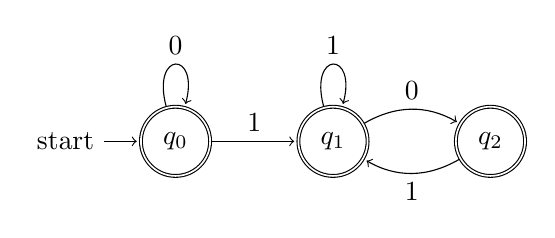
\begin{tikzpicture}[shorten >=1pt,node distance=2cm,on grid,auto]
        \node[state,initial,accepting]  (q_0)   {$q_0$};
        \node[state,accepting]          (q_1) [right=of q_0] {$q_1$};
        \node[state,accepting]          (q_2) [right=of q_1] {$q_2$};
        \path[->]
        (q_0)   edge    node    {$1$}   (q_1)
                edge    [loop above]    node    {$0$}   ()
        (q_1)   edge    [bend left]    node    {$0$}   (q_2)
                edge    [loop above]    node    {$1$}   ()
        (q_2)   edge    [bend left]    node    {$1$}   (q_1)
        ;
    \end{tikzpicture}
  \end{enumerate}

   \newpage


  \item \pts{$5\times 3=15$} Using the techniques covered in class, transform the following NFAs with $\epsilon$-transitions over the given alphabet $\Sigma$ into DFAs. Note that a DFA must have a transition defined for every state and symbol pair, whereas a NFA need not. You must take this fact into account for your transformations. Hint: Is there a subset of states the NFA transitions to when fed a symbol for which the set of current states has no explicit transition?

  \begin{enumerate}
    \item Original NFA, $\Sigma = \{a, b, c\}$:
    \\
    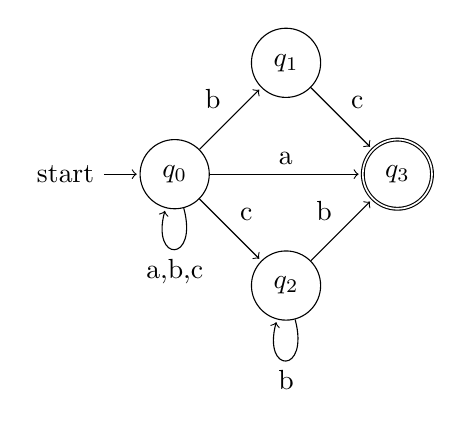
\begin{tikzpicture}[shorten >=1pt,node distance=2cm,on grid,auto]
        \node[state,initial]    (q_0)   {$q_0$};
        \node[state]            (q_1) [above right=of q_0] {$q_1$};
        \node[state]            (q_2) [below right=of q_0] {$q_2$};
        \node[state,accepting]  (q_3) [below right=of q_1] {$q_3$};
        \path[->]
        (q_0) edge [loop below] node {a,b,c} ()
              edge  node  [above] {a} (q_3)
              edge  node  {b} (q_1)
              edge  node  {c} (q_2)
        (q_1) edge  node  {c} (q_3)
        (q_2) edge  node  {b} (q_3)
              edge  [loop below] node  {b} ();
    \end{tikzpicture}
    \\
    DFA:
    \\
    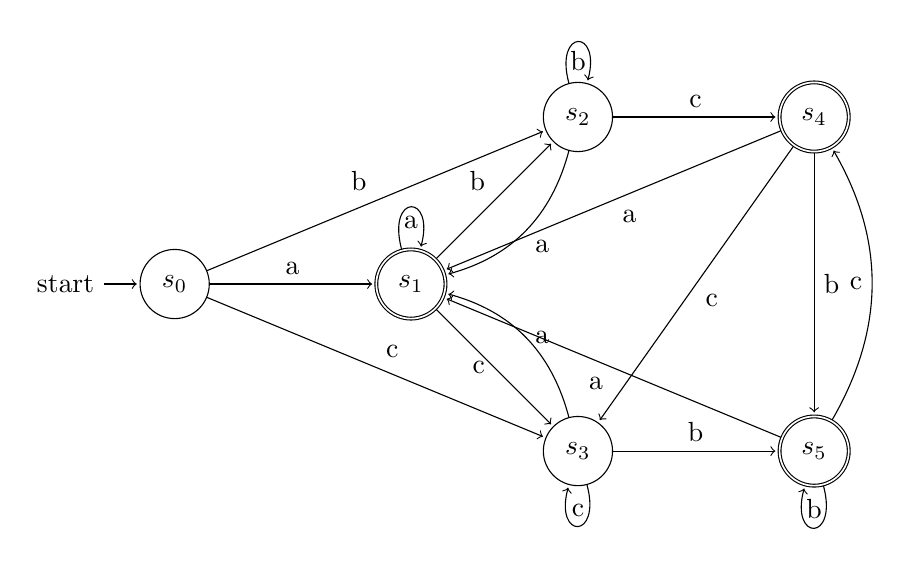
\begin{tikzpicture}[shorten >=1pt,node distance=3cm,on grid,auto]
        \node[state,initial]    (s_0)   {$s_0$};
        \node[state,accepting]  (s_1) [right=of s_0]   {$s_1$};
        \node[state]            (s_2) [above right=of s_1]   {$s_2$};
        \node[state]            (s_3) [below right=of s_1]   {$s_3$};
        \node[state,accepting]  (s_4) [right=of s_2]   {$s_4$};
        \node[state,accepting]  (s_5) [right=of s_3]   {$s_5$};
        \path[->]
        (s_0)   edge    node    {a} (s_1)
                edge    node    {b} (s_2)
                edge    node    {c} (s_3)
        (s_1)   edge    node    {b} (s_2)
                edge    node    [left]    {c} (s_3)
                edge    [loop above]    node    [below]    {a} ()
        (s_2)   edge    [bend left]    node    {a} (s_1)
                edge    node    {c} (s_4)
                edge    [loop above]    node    [below]    {b} ()
        (s_3)   edge    [bend right]    node    [right]    {a} (s_1)
                edge    node    {b} (s_5)
                edge    [loop below]    node    [above]    {c} ()
        (s_4)   edge    node    {a} (s_1)
                edge    node    {b} (s_5)
                edge    node    {c} (s_3)
        (s_5)   edge    node    {a} (s_1)
                edge    [bend right]    node    {c} (s_4)
                edge    [loop below]    node    [above]    {b} ()
        ;
    \end{tikzpicture}
    \item Original NFA, $\Sigma = \{a, b, c\}$:
    \\
    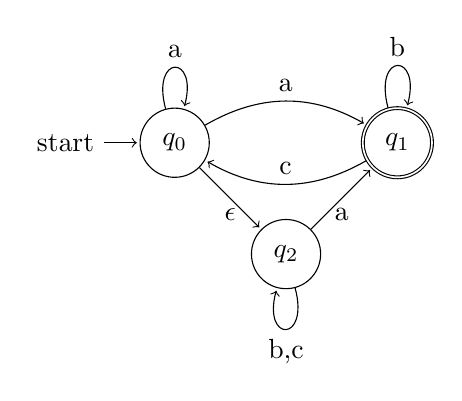
\begin{tikzpicture}[shorten >=1pt,node distance=2cm,on grid,auto]
        \node[state,initial]    (q_0)   {$q_0$};
        \node[state]            (q_2) [below right=of q_0] {$q_2$};
        \node[state,accepting]  (q_1) [above right=of q_2] {$q_1$};
        \path[->]
        (q_0) edge [loop above] node {a} ()
              edge [bend left] node  {a} (q_1)
              edge  node [below] {$\epsilon$} (q_2)
        (q_1) edge [loop above] node {b} ()
              edge [bend left] node [above] {c} (q_0)
        (q_2) edge node [below] {a} (q_1)
              edge [loop below] node  {b,c} ();
    \end{tikzpicture}
    \\
    DFA:
    \\
    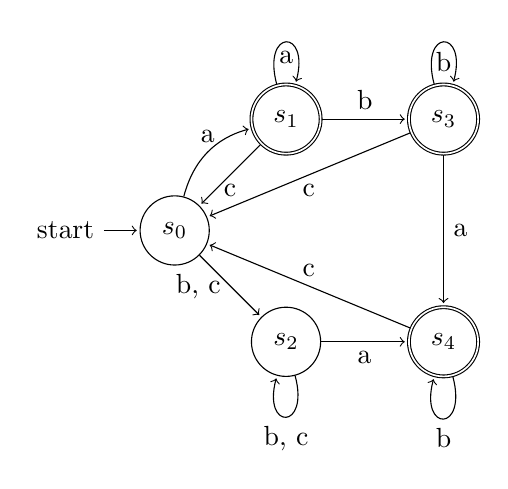
\begin{tikzpicture}[shorten >=1pt,node distance=2cm,on grid,auto]
        \node[state, initial] 	(s_0) 						{$s_0$};
        \node[state, accepting] (s_1) [above right=of s_0]	{$s_1$};
        \node[state] 			(s_2) [below right=of s_0] 	{$s_2$};
        \node[state, accepting] (s_3) [right=of s_1] 			{$s_3$};
        \node[state, accepting] (s_4) [right=of s_2] 			{$s_4$};
        \path[->]
        (s_0) 	edge 	[bend left]    node 	[above] 	{a} (s_1)
                edge 	node 	[left]		{b, c}  (s_2)
        (s_1) 	edge 	node 	[below] 	{c} 	(s_0)
                edge 	[loop above] 	node 	[below]		{a}		()
                edge 	node 	{b}	(s_3)
        (s_2) 	edge 	[loop below] 	node 	[below] 	{b, c} 	()
                edge 	node 	[below]		{a} (s_4)
        (s_3) 	edge 	node 	[below] 	{c} (s_0)
                edge 	[loop above] 	node 	[below] 	{b} 	()
                edge 	node 	{a} (s_4)
        (s_4) 	edge 	[loop below] 	node 	[below] 	{b} 	()
                edge 	node 	[above] 	{c} 	(s_0);
    \end{tikzpicture}
    \item Original NFA, $\Sigma = \{a, b,c\}$:
    \\
    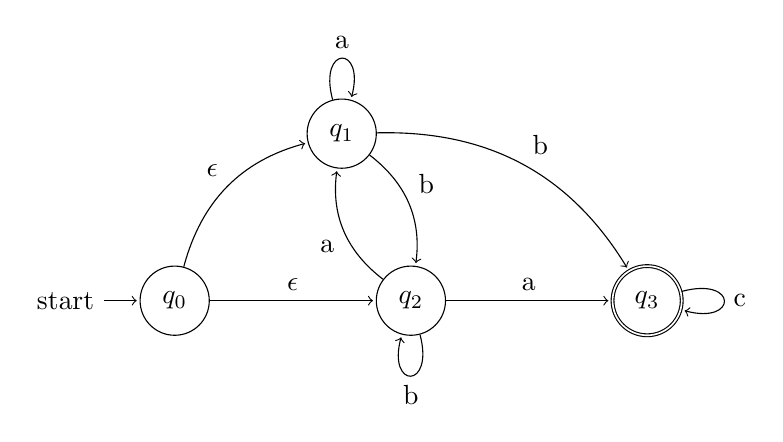
\begin{tikzpicture}[shorten >=1pt,node distance=3cm,on grid,auto]
        \node[state,initial] (q_0)   {$q_0$};
        \node[state] (q_1) [above right=of q_0] {$q_1$};
        \node[state] (q_2) [right=of q_0] {$q_2$};
        \node[state,accepting] (q_3) [right=of q_2] {$q_3$};
        \path[->]
        (q_0) edge [bend left] node  {$\epsilon$} (q_1)
              edge node  {$\epsilon$} (q_2)
        (q_1) edge [loop above] node {a} ()
              edge [bend left] node {b} (q_3)
              edge [bend left] node {b} (q_2)
        (q_2) edge [loop below] node {b} ()
              edge node {a} (q_3)
              edge [bend left] node {a} (q_1)
        (q_3) edge [loop right] node {c} ();
    \end{tikzpicture}
    \\
    DFA:
    \\
    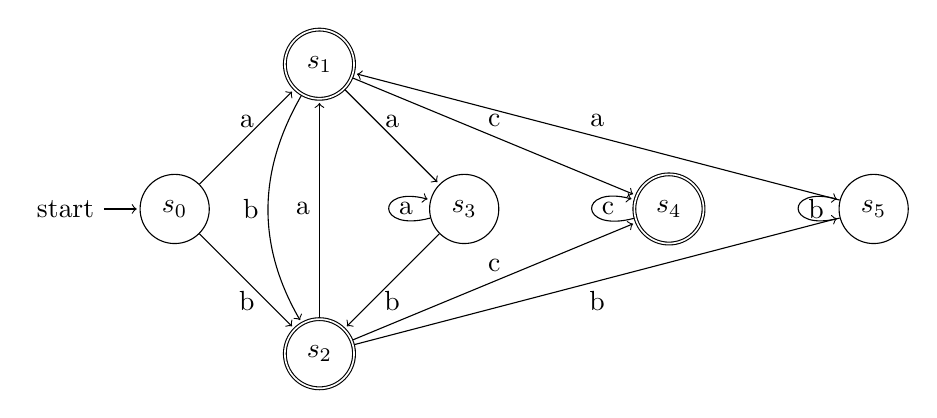
\begin{tikzpicture}[shorten >=1pt,node distance=2.6cm,on grid,auto]
        \node[state, initial] 	(s_0) 						{$s_0$};
        \node[state, accepting] (s_1) [above right=of s_0] 	{$s_1$};
        \node[state, accepting] (s_2) [below right=of s_0] 	{$s_2$};
        \node[state] 			(s_3) [below right=of s_1] 	{$s_3$};
        \node[state, accepting] (s_4) [right=of s_3] 		{$s_4$};
        \node[state] 			(s_5) [right=of s_4] 	    {$s_5$};

        \path[->]
        (s_0) 	edge 	node 	[above] 	{a} 	(s_1)
                edge 	node 	[below] 	{b}		(s_2)
        (s_1) 	edge 	[bend right] 	node 	[left]	 	{b}		(s_2)
                edge 	node 	[above] 	{a} 	(s_3)
                edge 	node 	[above] 	{c} 	(s_4)
        (s_2)	edge 	node 	[left] 	{a} 	(s_1)
                edge	node 	[below] 	{b} 	(s_5)
                edge 	node 	[above] 	{c} 	(s_4)
        (s_3) 	edge 	[loop left] 	node 	[right] 		{a} 	()
                edge 	node 	[below]		{b}		(s_2)
        (s_5) 	edge	node 	[above] 	{a} 	(s_1)
                edge 	[loop left] 	node 	[right] 	{b} 	()
        (s_4) 	edge 	[loop left] 	node 	[right] 	{c} 	();
    \end{tikzpicture}
  \end{enumerate}

   \newpage
  \item \pts{$13$} Draw the NFA for the set of all strings over the alphabet $\Sigma = \{a,b\}$, where both $a$ and $b$ occur even times.
Examples of strings that should be accepted by this NFA: abbabbbbaa, baabaaabaaaaab.
Examples of strings that should \textbf{not} be accepted: ababb, abbbabba.
    \\
    \\
    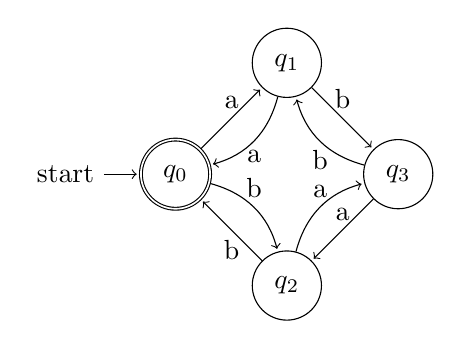
\begin{tikzpicture}[shorten >=1pt,node distance=2cm,on grid,auto]
        \node[state, initial, accepting] 	(q_0) 		{$q_0$};
        \node[state] 	(q_1)	[above right=of q_0]		{$q_1$};
        \node[state]	(q_2) 	[below right=of q_0]		{$q_2$};
        \node[state] 	(q_3) 	[below right=of q_1] 	{$q_3$};
        \path[->]
        (q_0)	edge 	node 	[above] 	{a} 	(q_1)
                edge 	[bend left]		node 	[above]		{b}	 	(q_2)
        (q_1) 	edge	[bend left] 	node 	[below] 	{a}		(q_0)
                edge 	node 	[above]		{b}		(q_3)
        (q_2) 	edge 	node 	[below] 	{b}	 	(q_0)
                edge 	[bend left]		node 	[above] 	{a}		(q_3)
        (q_3)	edge 	node 	[above] 	{a} 	(q_2)
                edge 	[bend left]		node 	[below] 	{b}		(q_1);
    \end{tikzpicture}\\
    where $q_0$ denotes even a and even b,
          $q_1$ denotes odd a and even b,
          $q_2$ denotes even a and odd b,
          $q_2$ denotes odd a and odd b,
  \newpage
   \item \pts{$5$} Consider the following tokens and their associated regular expressions, given as a \textbf{flex} scanner specification:

  \begin{lstlisting}
    %%
    (if)                    {printf("IF");}
    (0*1|1*0)               {printf("PS");}
    [0-9]+                  {printf("NUM");}
    [a-zA-Z0-9]+            {printf("ID");}
    [ ]                     {}
  \end{lstlisting}

  Give an input to this scanner such that the output string is $\tt (NUM^{\rm 2} IF^{\rm 2} ID^{\rm 3} PS)^{\rm 2}$, where $\tt A^i$ denotes {\tt A} repeated {\tt i} times.   (And, of course, the parentheses are not part of the output.)  You may use similar shorthand notation in your answer.
  \[
      ((2\ )^2(if\ )^2(a\ )^31\ )^2
  \]

  \newpage
  \item \pts{$5$} Draw the minimal DFA of the DFA constructed in Question 4(c).
   \\
    \\
    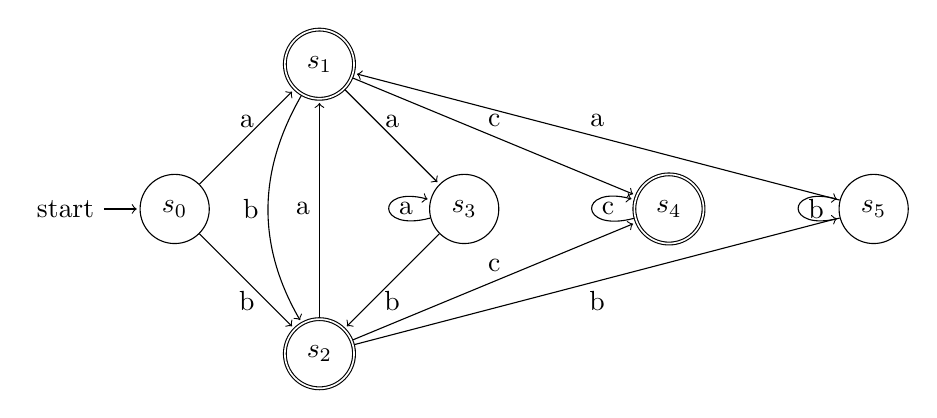
\begin{tikzpicture}[shorten >=1pt,node distance=2.6cm,on grid,auto]
        \node[state, initial] 	(s_0) 						{$s_0$};
        \node[state, accepting] (s_1) [above right=of s_0] 	{$s_1$};
        \node[state, accepting] (s_2) [below right=of s_0] 	{$s_2$};
        \node[state] 			(s_3) [below right=of s_1] 	{$s_3$};
        \node[state, accepting] (s_4) [right=of s_3] 		{$s_4$};
        \node[state] 			(s_5) [right=of s_4] 	    {$s_5$};

        \path[->]
        (s_0) 	edge 	node 	[above] 	{a} 	(s_1)
                edge 	node 	[below] 	{b}		(s_2)
        (s_1) 	edge 	[bend right] 	node 	[left]	 	{b}		(s_2)
                edge 	node 	[above] 	{a} 	(s_3)
                edge 	node 	[above] 	{c} 	(s_4)
        (s_2)	edge 	node 	[left] 	{a} 	(s_1)
                edge	node 	[below] 	{b} 	(s_5)
                edge 	node 	[above] 	{c} 	(s_4)
        (s_3) 	edge 	[loop left] 	node 	[right] 		{a} 	()
                edge 	node 	[below]		{b}		(s_2)
        (s_5) 	edge	node 	[above] 	{a} 	(s_1)
                edge 	[loop left] 	node 	[right] 	{b} 	()
        (s_4) 	edge 	[loop left] 	node 	[right] 	{c} 	();
    \end{tikzpicture}
    It's already a minimal DFA.

\end{enumerate}
\end{document}
